%----------------------------------------------------------------------------
\chapter{Implementáció}\label{sect:Implement}
%----------------------------------------------------------------------------

Egy ilyen volumenű alkalmazásnak rengeteg követelményt kell teljesítenie, hiszen a cél nem más, mint a Microsoft Project funkcióinak leimplementálása. A következő fejezetben szeretném kifejteni ezeket a követelményeket, továbbá azt, hogy ezeket hogyan teljesítettem.
\section{Felépítés}

Szükséges számunkra, egy \textit{hierachia} megvalósítása a feladatok között azaz, hogy lehhesen összefogó szülőfeladatokat megadni, alfeladatokat adni egy feladatnak. Fontos, hogy ezek között a feladatok között meg lehessen adni \textit{függőségeket}, azaz meg lehessen mondani egy feladatnak, hogy csak akkor hajthatódjon végre, ha már egy bizonyos másik feladat is végrehajtódott. Akkor nem csak függőségeket, de \textit{errőforrásokat} is meg lehessen adni egy faladathoz, hiszen tudnunk kell, hogy milyen erőforrásszükséglettel kell, hogy rendelkezzen egy feladat. Ezeknek az erőforrásoknak kell legyen egy típusuk és egy számuk, mely a rendelkezésre állásukat reprezentálja. Ezeken kívül szükségünk van egy \textit{munkanaptárra}, hisz ez alapján tudjuk megmondani, hogy milyen munkarend szerint zajlik a munka. Itt fontos, hogy minden naphoz ezt a munkarendet külön be lehessen állítani. Végül pedig már csak egy \textit{ütemezőre} van szükség, ami figyelembe véve a feladatokat megmondja, hogy melyiket mi után kell elvégeznünk optimálisan.

\begin{figure}[!ht]
\centering
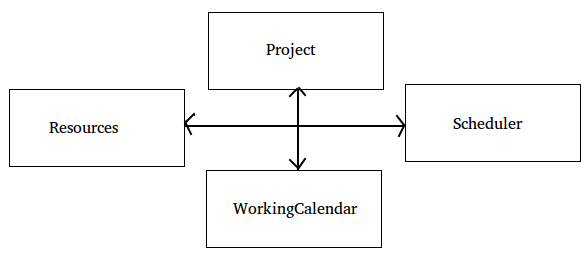
\includegraphics[width=\textwidth, keepaspectratio]{figures/project1.png}
\caption{Felépítés} 
\label{fig:project1}
\end{figure} 

Ezek alapján négy részből állítottam össze a programot, amik mindent tudnak egymásról, és folyamatosan kommunikálnak:
\begin{itemize}
	\item \textbf(Project:) A feladatokat, függőségeket és összefoglalókat (summaryket) megvalósító osztályok, illetve amik hozzájuk kapcsolódnak.
	\item \textbf(Resources:) Az erőforrások kezelését megvalósító komponens
	\item \textbf(Scheduler:) Az ütemező osztály, a feladatok ismeretével és a munkanaptár segítségével minden feladathoz hozzárendel egy időtartamot, amikor azt végre kell hajtani
	\item \textbf(WorkingCalendar:) Ez az ostály tartja nyilván a munkanapokat egy munkanaptáron keresztül, ez az osztály felelős a munkarendért
\end{itemize}

%----------------------------------------------------------------------------
\section{Project}

%----------------------------------------------------------------------------
\section{WorkingCalendar}

%----------------------------------------------------------------------------
\section{Schedulers}

%----------------------------------------------------------------------------
\section{Resources}
